\section{Particle analysis}
\label{sec:particle}


As in Figure \ref{fig:categorize_regions}, the solution space will be divided into three types of regions by the global best and the personal best.
\begin{itemize}
\item $ f(x) > f(x^G) $
Once a particle gets into this region, it updates both global best and personal best. 
It becomes a leader of the swarm.
\item $ f(x^{G}) > f(x) > f(x^{P}) $
Once a particle gets into this region, it updates only the personal best.
The solution space is then re-divided.
\item $ f(x) < f(x^{P}) $
When a particle is in this region, it only moves as a random walk.
\end{itemize}

\begin{figure}
\centering
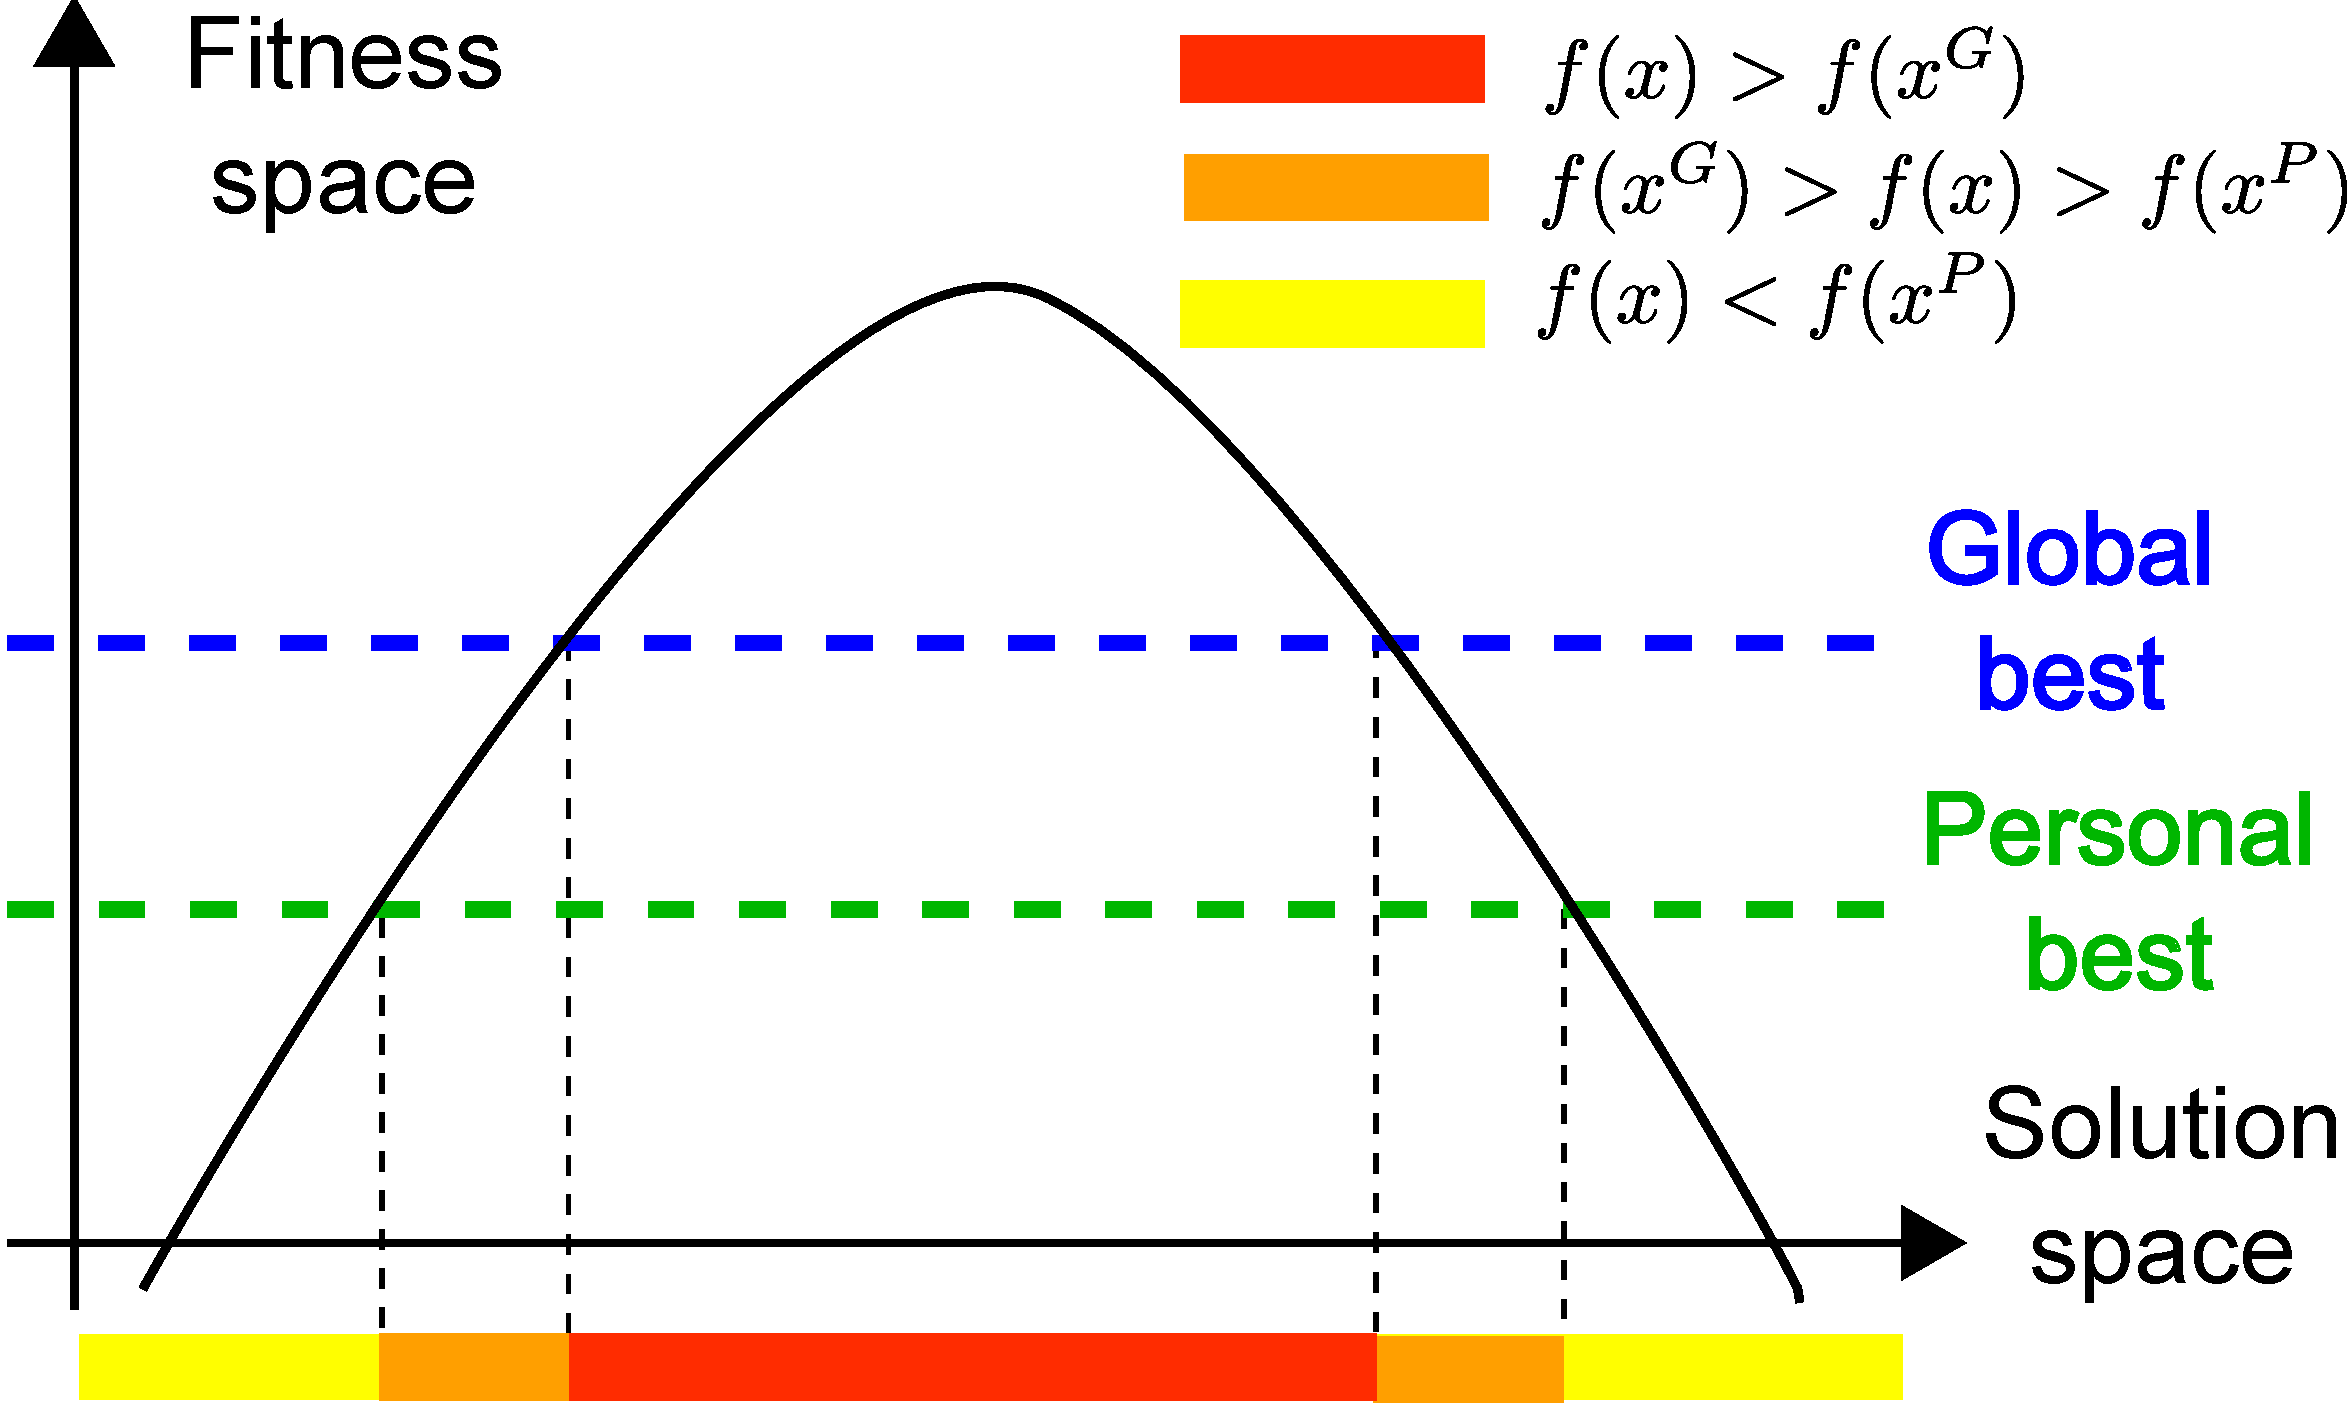
\includegraphics[width=0.7\linewidth]{./fig/categorize_regions}
\caption{How global best and personal best divide the solution space.}
\label{fig:categorize_regions}
\end{figure}

The result of the movement of a particle is determined by which region of the solution space it moves in.

\subsection{What happens in a single hill case}

When the fitness distribution is a single hill, the analysis can be easier.
In most of the cases, the particles should all converge into a single hill where the global best locates in.

\begin{myprop}
In a single hill case, $ x^{p}(k) = x(k) $. 
\end{myprop}

It means that there is no effect from a personal best.p
[TODO] random walk reaching a point


\begin{mylem}
In a single hill case, when $ x^{G} = x^{*} $, the particle will converge to $ x^{G} $ if the particle is ISS.
\end{mylem}

\begin{mylem}
In a single hill case, when $ f( x^{G} ) < f( x^{*}) $, the particle will converge to $ \hat{x^{*}} $ and $ f(\hat{x^{*}}) \geq f(x^{G}) $ if the particle is ISS.
The probability of $ \hat{x^{*}} = x^{G} $ is .
\end{mylem}

\begin{figure}[ht]
\centering
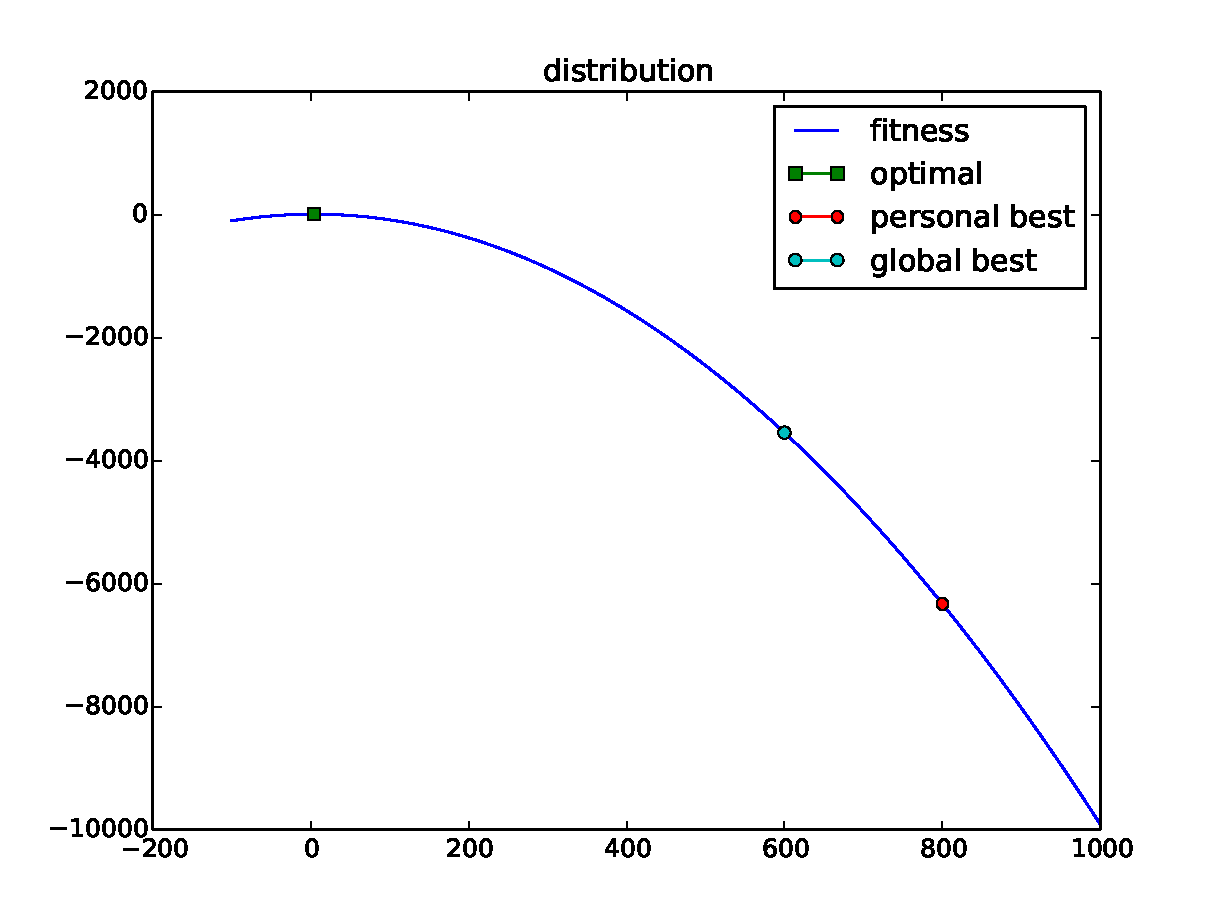
\includegraphics[width=.7\linewidth]{./simfig/case1/distribution1}
\label{fig:case1-1:distribution} 
\end{figure}

\begin{figure}[ht]
\centering
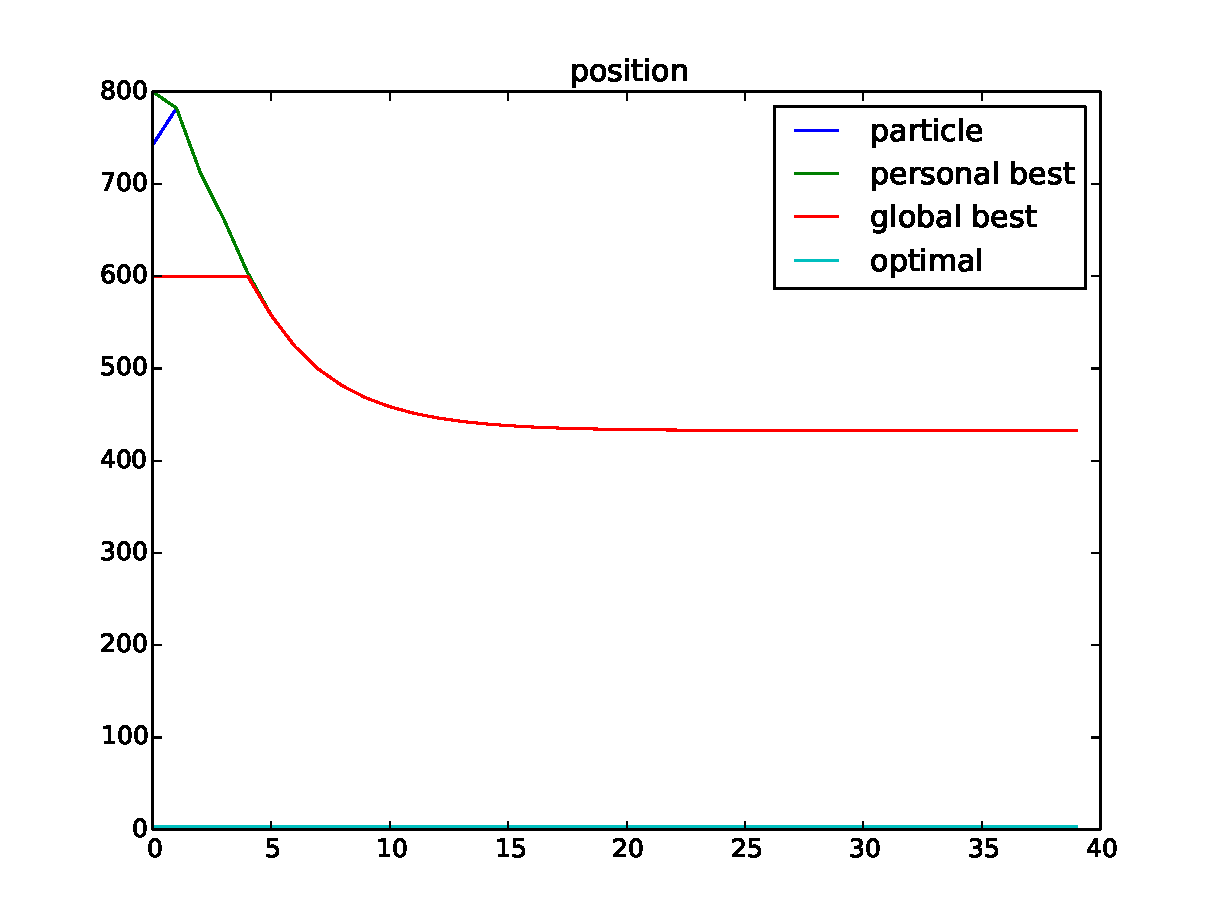
\includegraphics[width=.7\linewidth]{./simfig/case1/position1-1} 
\label{fig:case1-1:position}
\caption{$ \chi = 0.72984 , \phi^{P} = 2.05 , \phi^{G} = 2.05 $ }
\end{figure}

\begin{figure}[ht]
\centering
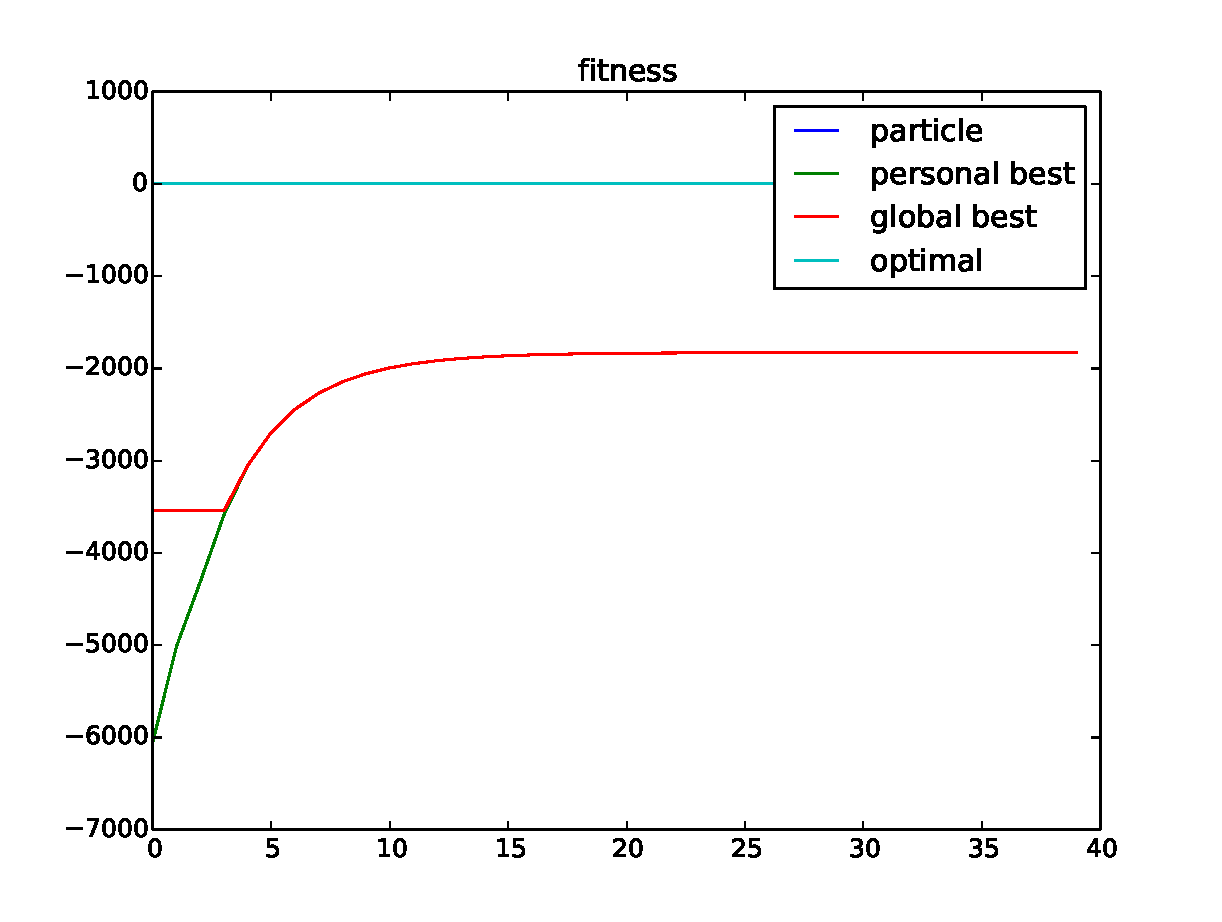
\includegraphics[width=.7\linewidth]{./simfig/case1/fitness1-1} 
\label{fig:case1-1:fitness}
\caption{$ \chi = 0.72984 , \phi^{P} = 2.05 , \phi^{G} = 2.05 $ }
\end{figure}

\begin{figure}[ht]
\centering
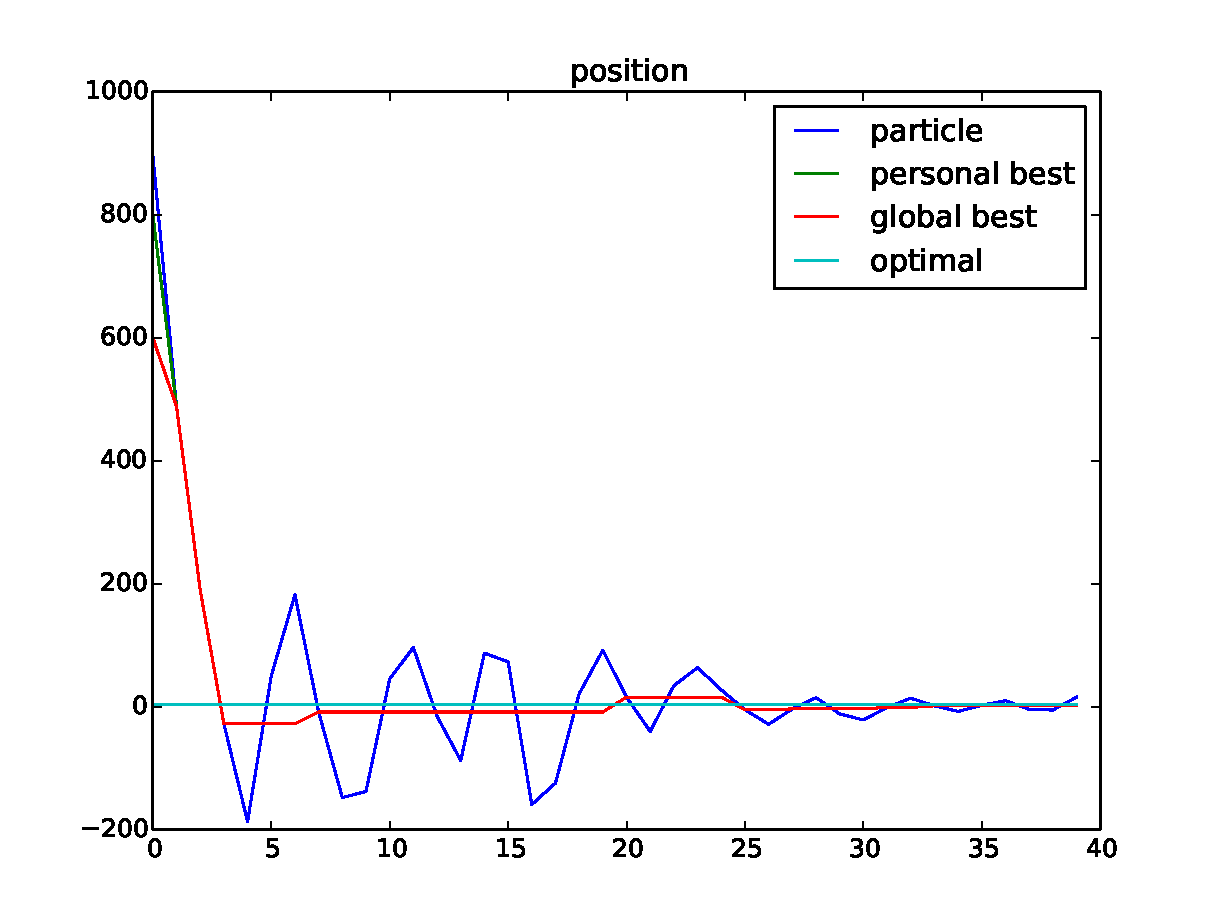
\includegraphics[width=.7\linewidth]{./simfig/case1/position1-2} 
\label{fig:case1-2:position}
\caption{$ \chi = 0.72984 , \phi^{P} = 2.05 , \phi^{G} = 2.05 $ }
\end{figure}
  
\begin{figure}[ht]
\centering
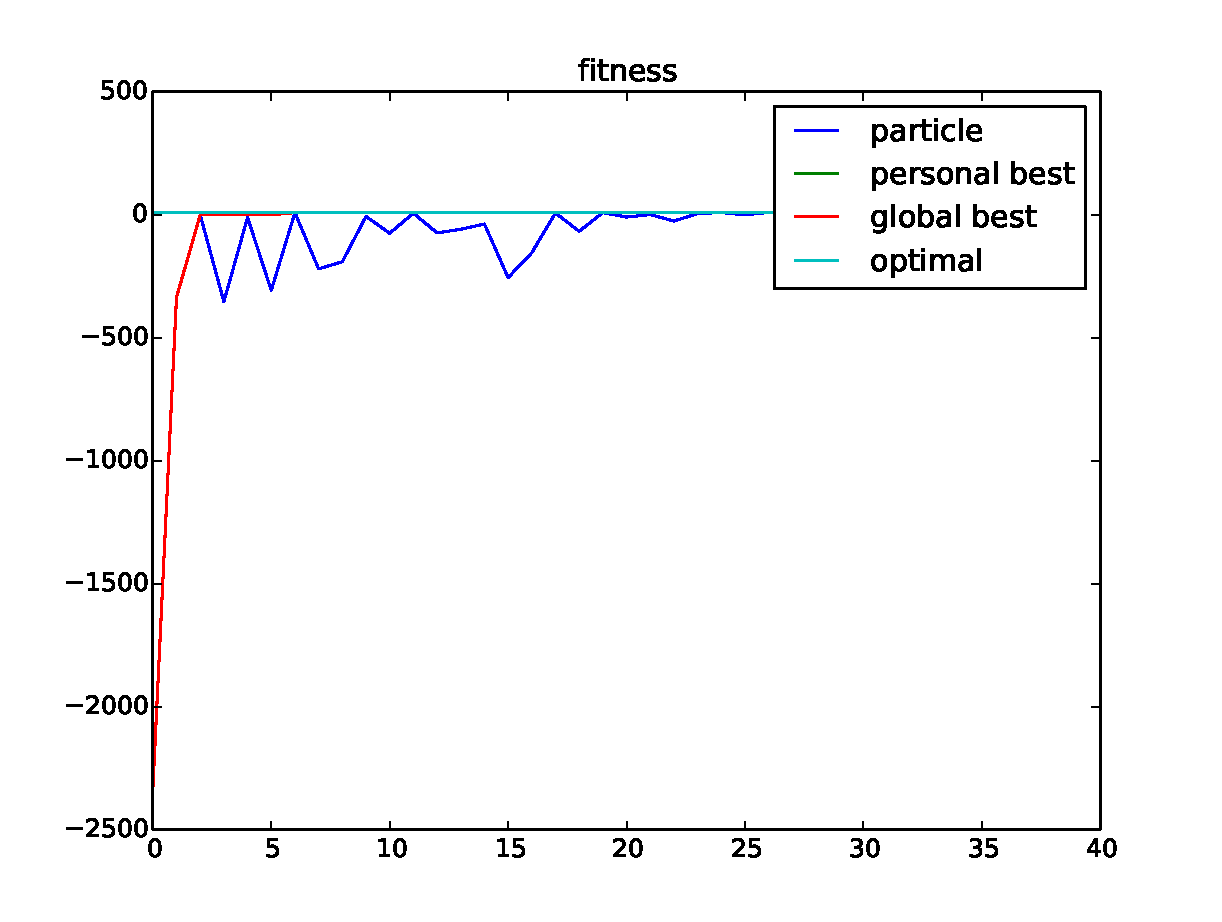
\includegraphics[width=.7\linewidth]{./simfig/case1/fitness1-2} 
\label{fig:case1-2:fitness} 
\caption{$ \chi = 0.72984 , \phi^{P} = 2.05 , \phi^{G} = 2.05 $ }
\end{figure}


\subsection{More than single hill case}


\begin{figure}[ht]
\centering
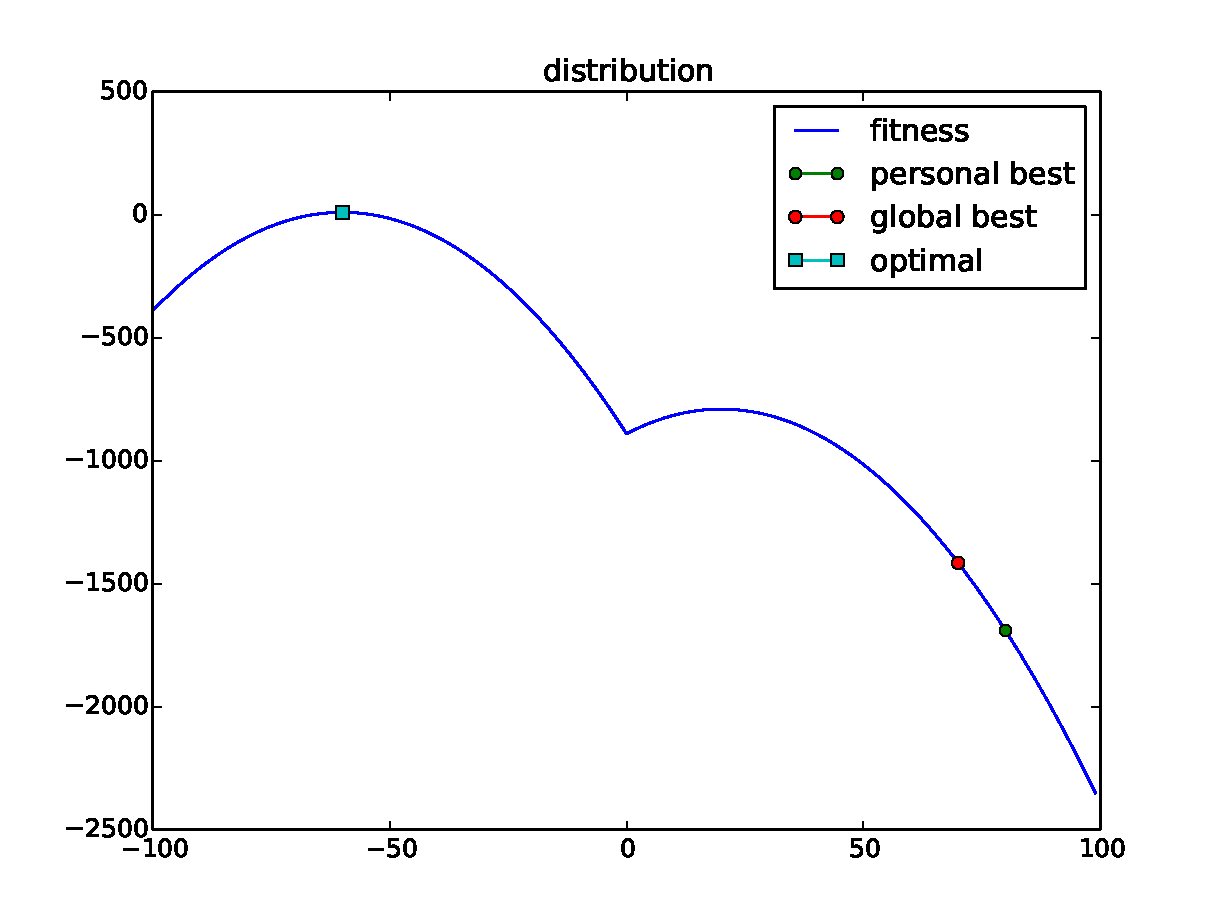
\includegraphics[width=.7\linewidth]{./simfig/case2/distribution2}
\label{fig:case2-1:distribution} 
\end{figure}

\begin{figure}[ht]
\centering
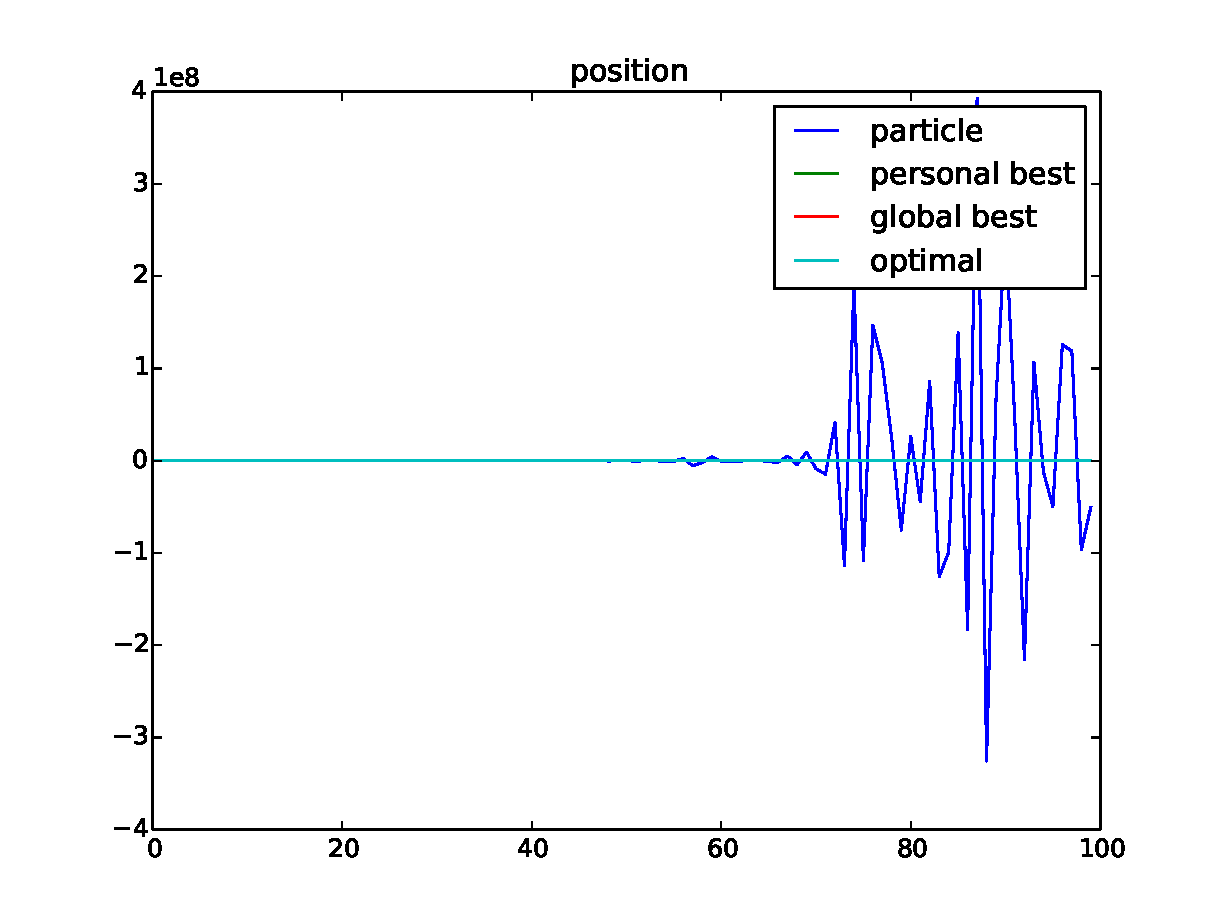
\includegraphics[width=.7\linewidth]{./simfig/case2/position2-1} 
\label{fig:case2-1:position}
\caption{$ \chi = 0.72984 , \phi^{P} = 2.05 , \phi^{G} = 2.05 $ }
\end{figure}

\begin{figure}[ht]
\centering
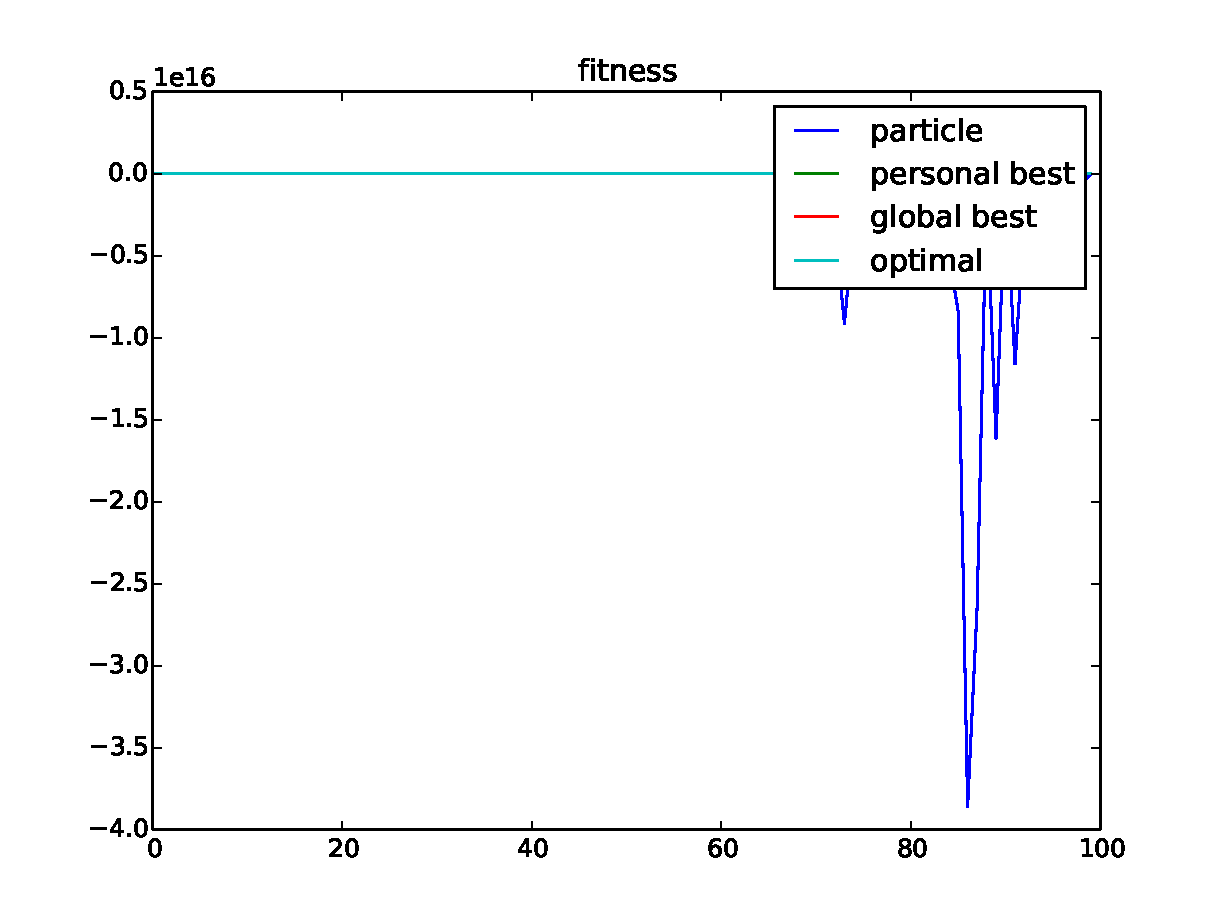
\includegraphics[width=.7\linewidth]{./simfig/case2/fitness2-1} 
\label{fig:case2-1:fitness}
\caption{$ \chi = 0.72984 , \phi^{P} = 2.05 , \phi^{G} = 2.05 $ }
\end{figure}

\begin{figure}[ht]
\centering
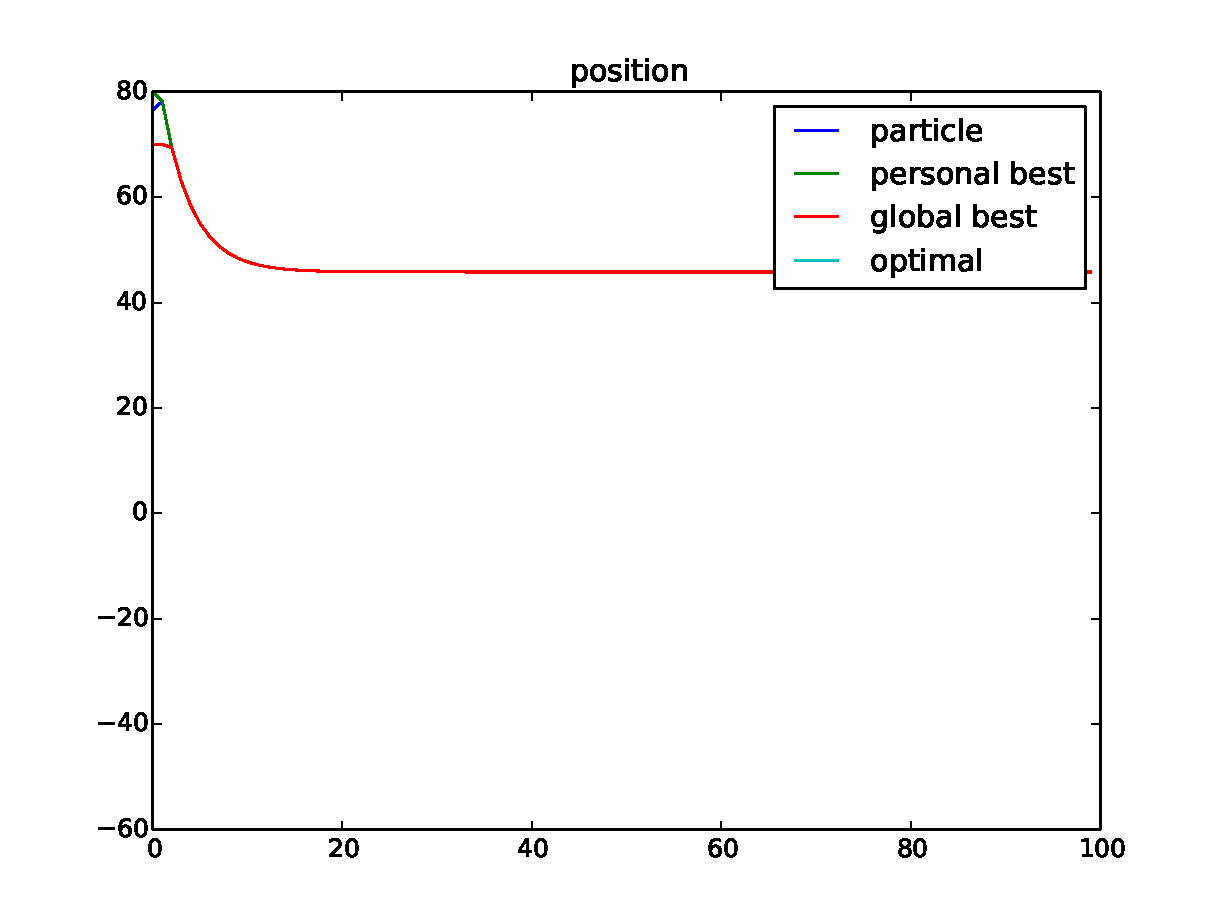
\includegraphics[width=.7\linewidth]{./simfig/case2/position2-2} 
\label{fig:case2-2:position}
\caption{$ \chi = 0.72984 , \phi^{P} = 2.05 , \phi^{G} = 2.05 $ }
\end{figure}
  
\begin{figure}[ht]
\centering
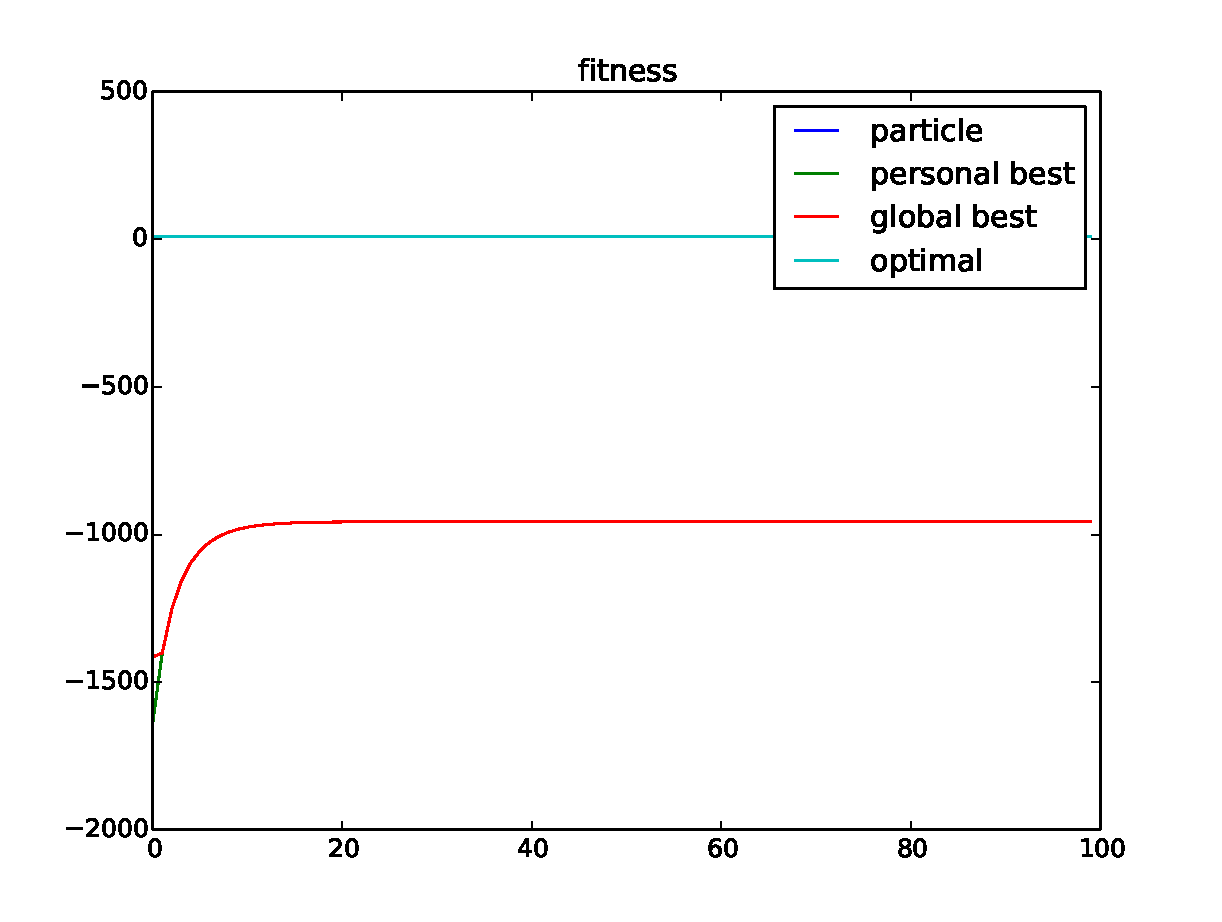
\includegraphics[width=.7\linewidth]{./simfig/case2/fitness2-2} 
\label{fig:case2-2:fitness} 
\caption{$ \chi = 0.72984 , \phi^{P} = 2.05 , \phi^{G} = 2.05 $ }
\end{figure}

